% Copyright (c) 2020 Matematyka dla Ciekawych Świata (http://ciekawi.icm.edu.pl/)
% Copyright (c) 2020 Robert Ryszard Paciorek <rrp@opcode.eu.org>
% Copyright (c) 2020 Krzysztof Lasocki <krz.lasocki@gmail.com>
% 
% MIT License
% 
% Permission is hereby granted, free of charge, to any person obtaining a copy
% of this software and associated documentation files (the "Software"), to deal
% in the Software without restriction, including without limitation the rights
% to use, copy, modify, merge, publish, distribute, sublicense, and/or sell
% copies of the Software, and to permit persons to whom the Software is
% furnished to do so, subject to the following conditions:
% 
% The above copyright notice and this permission notice shall be included in all
% copies or substantial portions of the Software.
% 
% THE SOFTWARE IS PROVIDED "AS IS", WITHOUT WARRANTY OF ANY KIND, EXPRESS OR
% IMPLIED, INCLUDING BUT NOT LIMITED TO THE WARRANTIES OF MERCHANTABILITY,
% FITNESS FOR A PARTICULAR PURPOSE AND NONINFRINGEMENT. IN NO EVENT SHALL THE
% AUTHORS OR COPYRIGHT HOLDERS BE LIABLE FOR ANY CLAIM, DAMAGES OR OTHER
% LIABILITY, WHETHER IN AN ACTION OF CONTRACT, TORT OR OTHERWISE, ARISING FROM,
% OUT OF OR IN CONNECTION WITH THE SOFTWARE OR THE USE OR OTHER DEALINGS IN THE
% SOFTWARE.

\documentclass{pdfBooklets}

\title{Warsztat Elektroniczny}
\author{%
	Projekt ,,Matematyka dla Ciekawych Świata'',\\
	Krzysztof Lasocki\\\normalsize\ttfamily <krz.lasocki@gmail.com>,\\
	Robert Ryszard Paciorek \normalsize\ttfamily <rrp@opcode.eu.org>
}
\date  {2023-06-25}

\makeatletter\hypersetup{
	pdftitle = {\@title}, pdfauthor = {\@author}
}\makeatother

% Copyright (c) 2017-2020 Matematyka dla Ciekawych Świata (http://ciekawi.icm.edu.pl/)
% Copyright (c) 2017-2020 Robert Ryszard Paciorek <rrp@opcode.eu.org>
% Copyright (c) 2020 Krzysztof Lasocki <krz.lasocki@gmail.com>
% 
% MIT License
% 
% Permission is hereby granted, free of charge, to any person obtaining a copy
% of this software and associated documentation files (the "Software"), to deal
% in the Software without restriction, including without limitation the rights
% to use, copy, modify, merge, publish, distribute, sublicense, and/or sell
% copies of the Software, and to permit persons to whom the Software is
% furnished to do so, subject to the following conditions:
% 
% The above copyright notice and this permission notice shall be included in all
% copies or substantial portions of the Software.
% 
% THE SOFTWARE IS PROVIDED "AS IS", WITHOUT WARRANTY OF ANY KIND, EXPRESS OR
% IMPLIED, INCLUDING BUT NOT LIMITED TO THE WARRANTIES OF MERCHANTABILITY,
% FITNESS FOR A PARTICULAR PURPOSE AND NONINFRINGEMENT. IN NO EVENT SHALL THE
% AUTHORS OR COPYRIGHT HOLDERS BE LIABLE FOR ANY CLAIM, DAMAGES OR OTHER
% LIABILITY, WHETHER IN AN ACTION OF CONTRACT, TORT OR OTHERWISE, ARISING FROM,
% OUT OF OR IN CONNECTION WITH THE SOFTWARE OR THE USE OR OTHER DEALINGS IN THE
% SOFTWARE.

\usepackage{tikz}
\usetikzlibrary{circuits.ee.IEC}

\newtcolorbox{Ramka}[1][]{
	colback=white,
	colbacktitle=white,
	coltitle=black,
	colframe=white!50!black,
	fontupper=\small,
	enhanced,
	before skip=13pt plus 2pt,
	#1
}

% Symbol DC
\newcommand{\mathdirectcurrent}{\mathrel{\mathpalette\mathdirectcurrentinner\relax}}
\newcommand{\mathdirectcurrentinner}[2]{%
  \settowidth{\dimen0}{$#1=$}%
  \vbox to .85ex {\offinterlineskip
    \hbox to \dimen0{\hss\leaders\hrule\hskip.85\dimen0\hss}
    \vskip.35ex
    \hbox to \dimen0{\hss
      \leaders\hrule\hskip.17\dimen0
      \hskip.17\dimen0
      \leaders\hrule\hskip.17\dimen0
      \hskip.17\dimen0
      \leaders\hrule\hskip.17\dimen0
    \hss}
    \vfill
  }%
}
% symbol diody
\newcommand\esymbol[1]{\tikz[circuit ee IEC] \draw (0,0) -- (.1,0) node [#1,anchor=west,name=s] {} (s.east) -- +(.1,0);}

\newcommand{\textdirectcurrent}{\mathdirectcurrentinner{\textstyle}{}}

\newcommand\zaleta{\item[\textbf{\ttfamily +}]}
\newcommand\wada{\item[\textbf{\ttfamily -}]}
\newcommand\info{\item[\textbf{\ttfamily *}]}
\newcommand\uwaga{\item[\textbf{\ttfamily !}]}


\begin{document}

\maketitle

% Copyright (c) 2021 Robert Ryszard Paciorek <rrp@opcode.eu.org>
% 
% MIT License
% 
% Permission is hereby granted, free of charge, to any person obtaining a copy
% of this software and associated documentation files (the "Software"), to deal
% in the Software without restriction, including without limitation the rights
% to use, copy, modify, merge, publish, distribute, sublicense, and/or sell
% copies of the Software, and to permit persons to whom the Software is
% furnished to do so, subject to the following conditions:
% 
% The above copyright notice and this permission notice shall be included in all
% copies or substantial portions of the Software.
% 
% THE SOFTWARE IS PROVIDED "AS IS", WITHOUT WARRANTY OF ANY KIND, EXPRESS OR
% IMPLIED, INCLUDING BUT NOT LIMITED TO THE WARRANTIES OF MERCHANTABILITY,
% FITNESS FOR A PARTICULAR PURPOSE AND NONINFRINGEMENT. IN NO EVENT SHALL THE
% AUTHORS OR COPYRIGHT HOLDERS BE LIABLE FOR ANY CLAIM, DAMAGES OR OTHER
% LIABILITY, WHETHER IN AN ACTION OF CONTRACT, TORT OR OTHERWISE, ARISING FROM,
% OUT OF OR IN CONNECTION WITH THE SOFTWARE OR THE USE OR OTHER DEALINGS IN THE
% SOFTWARE.

Istnieje co najmniej kilka dziedzin techniki związanych z prądem elektrycznym i jego wykorzystaniem (elektrotechnika, elektronika, elektroenergetyki, ...).
Granice pomiędzy nimi bywają niekiedy dość płynne (np. stosowanie elementów elektronicznych w zastosowaniach elektroenergetyki), gdyż wszystkie zajmują się zjawiskami związanymi z przepływem prądu elektrycznego, a typowo rozróżnia je wartość prądu, napięcia, mocy (tu jednak nie ma wyraźnych granic) oraz cel w jakim ten prąd ma płynąć (przekazanie sygnału czy wykonanie pracy).

W tym artykule poruszone zostaną kwestie, które niekoniecznie mają znaczenie w niskonapięciowej elektronice cyfrowej, za to są istotnymi aspektami w instalacjach elektrycznych.


% Copyright (c) 2017-2020 Matematyka dla Ciekawych Świata (http://ciekawi.icm.edu.pl/)
% Copyright (c) 2017-2020 Robert Ryszard Paciorek <rrp@opcode.eu.org>
% 
% MIT License
% 
% Permission is hereby granted, free of charge, to any person obtaining a copy
% of this software and associated documentation files (the "Software"), to deal
% in the Software without restriction, including without limitation the rights
% to use, copy, modify, merge, publish, distribute, sublicense, and/or sell
% copies of the Software, and to permit persons to whom the Software is
% furnished to do so, subject to the following conditions:
% 
% The above copyright notice and this permission notice shall be included in all
% copies or substantial portions of the Software.
% 
% THE SOFTWARE IS PROVIDED "AS IS", WITHOUT WARRANTY OF ANY KIND, EXPRESS OR
% IMPLIED, INCLUDING BUT NOT LIMITED TO THE WARRANTIES OF MERCHANTABILITY,
% FITNESS FOR A PARTICULAR PURPOSE AND NONINFRINGEMENT. IN NO EVENT SHALL THE
% AUTHORS OR COPYRIGHT HOLDERS BE LIABLE FOR ANY CLAIM, DAMAGES OR OTHER
% LIABILITY, WHETHER IN AN ACTION OF CONTRACT, TORT OR OTHERWISE, ARISING FROM,
% OUT OF OR IN CONNECTION WITH THE SOFTWARE OR THE USE OR OTHER DEALINGS IN THE
% SOFTWARE.

\section{Zakupy, czyli co warto kupić na początek}

Praktyczna zabawa z elektroniką wymaga posiadania przynajmniej minimalnego zaplecza sprzętowego.
W jego skład powinno wejść co najmniej:
	uniwersalny miernik wielkości elektrycznych (multimetr),
	źródło zasilania (najlepiej z regulacją napięcia i ograniczenia prądowego),
	płytka prototypowa wraz z różnymi kabelkami i podstawowymi narzędziami (przynajmniej śrubokrętem),
	moduł mikrokontrolera wraz z programatorem
	oraz jakiś zestaw podstawowych elementów od których zaczniemy naszą zabawę.
W tym rozdziale powiemy na co warto zwrócić uwagę przy tych zakupach oraz przedstawiami kilka godnych uwagi propozycji dostępnych na rynku.


% Copyright (c) 2017-2020 Matematyka dla Ciekawych Świata (http://ciekawi.icm.edu.pl/)
% Copyright (c) 2017-2020 Robert Ryszard Paciorek <rrp@opcode.eu.org>
% 
% MIT License
% 
% Permission is hereby granted, free of charge, to any person obtaining a copy
% of this software and associated documentation files (the "Software"), to deal
% in the Software without restriction, including without limitation the rights
% to use, copy, modify, merge, publish, distribute, sublicense, and/or sell
% copies of the Software, and to permit persons to whom the Software is
% furnished to do so, subject to the following conditions:
% 
% The above copyright notice and this permission notice shall be included in all
% copies or substantial portions of the Software.
% 
% THE SOFTWARE IS PROVIDED "AS IS", WITHOUT WARRANTY OF ANY KIND, EXPRESS OR
% IMPLIED, INCLUDING BUT NOT LIMITED TO THE WARRANTIES OF MERCHANTABILITY,
% FITNESS FOR A PARTICULAR PURPOSE AND NONINFRINGEMENT. IN NO EVENT SHALL THE
% AUTHORS OR COPYRIGHT HOLDERS BE LIABLE FOR ANY CLAIM, DAMAGES OR OTHER
% LIABILITY, WHETHER IN AN ACTION OF CONTRACT, TORT OR OTHERWISE, ARISING FROM,
% OUT OF OR IN CONNECTION WITH THE SOFTWARE OR THE USE OR OTHER DEALINGS IN THE
% SOFTWARE.

\begin{wrapfigure}{r}{5.5cm}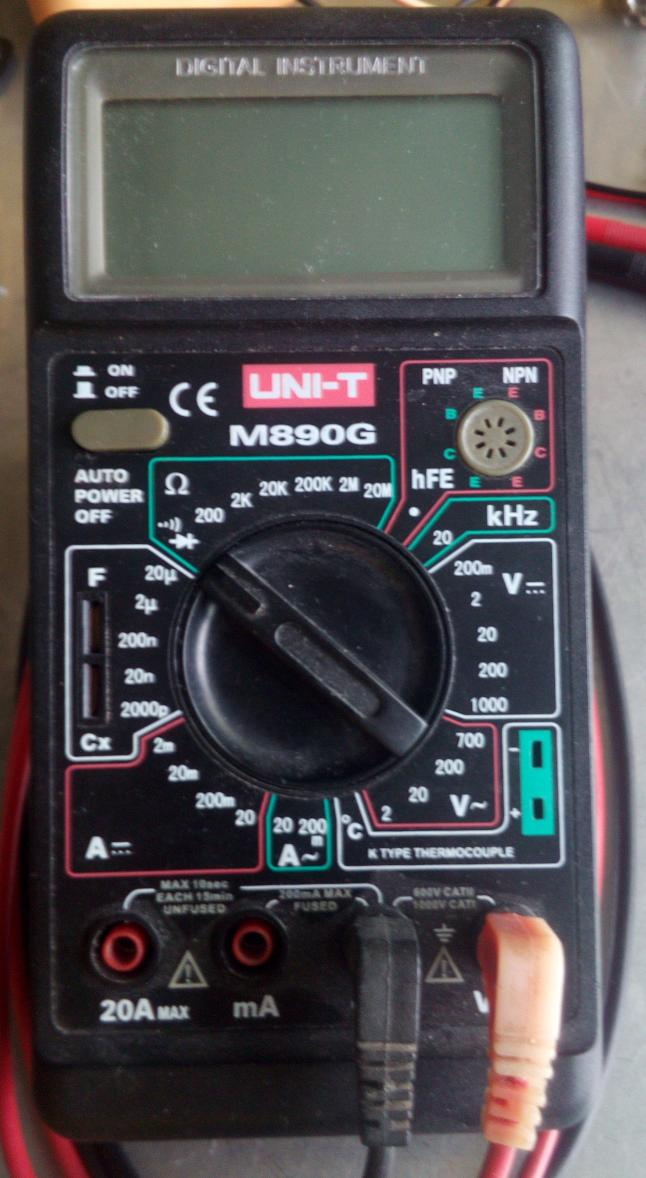
\includegraphics[width=5.5cm]{warsztat_elektroniczny/multimetr}\vspace{-1.2cm}\end{wrapfigure}

\subsection{Multimetr}

Najważniejszym przyrządem w naszym warsztacie elektronika jest uniwersalny miernik parametrów elektrycznych, zwany multimetrem.
Dla naszych potrzeb powinien on zapewniać co najmniej:
\begin{itemize}
	\item pomiar napięcia stałego (DC) od 0.1V do 20V (np. zakresy pomiarowe: 200mV, 20V)
	\item pomiar prądu stałego (DC) od 1mA do 200mA (np. zakresy pomiarowe: 20mA, 200mA)
	\item pomiar rezystancji od 10Ω do 1MΩ (np. zakresy pomiarowe: 200Ω, 20kΩ, 2000kΩ)
	\item pomiar diody
\end{itemize}

\noindent
Przydatne będą także funkcje takie jak:
\begin{itemize}
	\item  sygnalizacja akustyczna ciągłości obwodu (może być razem z pomiarem diody)
	\item pomiar tranzystora "hfe"
\end{itemize}
Oczywiście fajnie jak nasz miernik będzie miał szersze zakresy pomiarowe, będzie umożliwiał pomiar prądu zmiennego (AC), pojemności kondensatorów, itd., ale nie jest to wymagane.

Warto natomiast aby posiadał zabezpieczenie pomiaru prądu (czyli bezpiecznik w tym obwodzie, oznaczenie przy gniazdach "fused") przynajmniej na zakresie do 200mA.
Natomiast przy teście diody warto aby miernik podawał napięcie wystarczające, jeżeli nie do zmierzenia, to przynajmniej do zaświecenia dowolnego LED (czyli tak naprawdę białego lub niebieskiego).
	Niestety producenci na ogół nie podają tego parametru i nawet dobre mierniki potrafią mieć ten paramter zaskakująco słaby.

Ogólnie dobry multimetr jest ważny, ale na początek wystarczy nawet najtańszy model. Jeżeli będziemy kontynuować przygodę z elektroniką to z czasem i tak kupimy drugi, gdyż często przydaje się możliwość równoległego pomiaru w dwóch punktach, równoczesnego pomiaru prądu i napięcia, itd.

Poniżej kilka propozycji do wyboru.

\subsubsection{DT-830B /  DT-830D / DT-832 / DT-832D} (jest wiele bardzo zbliżonych modeli – warto zwrócić uwagę aby miał "fused" na zakresie 200mA oraz buzzer do sygnalizacji ciągłości obwodu)
	\begin{itemize}
		\zaleta spełnia wymagania minimalne oraz posiada pomiar hfe i test ciągłości obwodu
		\zaleta pomiar napięcia DC i AC do 500V
		\zaleta pomiar prądu DC do 10A
		\info od 10PLN
	\end{itemize}

\subsubsection{DT9205A}
	\begin{itemize}
		\zaleta spełnia wymagania minimalne oraz posiada pomiar hfe i test ciągłości obwodu
		\zaleta pomiar napięcia DC i AC do 500V
		\zaleta pomiar prądu DC i AC do 20A
		\zaleta pomiar pojemności
		\info od 20PLN
	\end{itemize}

\subsubsection{DT33A} (nie mylić z DT33B, DT33C i DT33D):
	\begin{itemize}
		\zaleta spełnia wymagania minimalne oraz posiada pomiar hfe i test ciągłości obwodu
		\zaleta pomiar napięcia DC i AC do 500V
		\zaleta pomiar prądu DC do 10A
		\zaleta pomiar pojemności
		\zaleta pomiar temperatury
		\info od 30PLN
	\end{itemize}

\subsubsection{DT890G / M890G / M890C}
	\begin{itemize}
		\zaleta spełnia wymagania minimalne oraz posiada pomiar hfe i test ciągłości obwodu
		\zaleta pomiar napięcia DC i AC do 500V
		\zaleta pomiar prądu DC i AC do 20A
		\zaleta pomiar pojemności
		\zaleta pomiar temperatury
		\zaleta pomiar częstotliwości (tylko DT890G / M890G)
		\zaleta (u niektórych producentów) zabezpieczony pomiar 20A
		\info od 35PLN
	\end{itemize}

\subsubsection{Uni-T UT890C+}
	\begin{itemize}
		\zaleta spełnia wymagania minimalne oraz posiada pomiar hfe i test ciągłości obwodu
		\zaleta pomiar napięcia DC i AC do 500V
		\zaleta pomiar prądu DC i AC do 20A
		\zaleta pomiar pojemności
		\zaleta pomiar temperatury
		\zaleta pomiar częstotliwości
		\zaleta zabezpieczony pomiar 20A
		\zaleta zakresy 6, 60, 600 a nie 2, 20, 200
		\zaleta true RMS
		\info od 76PLN
	\end{itemize}


% Copyright (c) 2017-2020 Matematyka dla Ciekawych Świata (http://ciekawi.icm.edu.pl/)
% Copyright (c) 2017-2020 Robert Ryszard Paciorek <rrp@opcode.eu.org>
% 
% MIT License
% 
% Permission is hereby granted, free of charge, to any person obtaining a copy
% of this software and associated documentation files (the "Software"), to deal
% in the Software without restriction, including without limitation the rights
% to use, copy, modify, merge, publish, distribute, sublicense, and/or sell
% copies of the Software, and to permit persons to whom the Software is
% furnished to do so, subject to the following conditions:
% 
% The above copyright notice and this permission notice shall be included in all
% copies or substantial portions of the Software.
% 
% THE SOFTWARE IS PROVIDED "AS IS", WITHOUT WARRANTY OF ANY KIND, EXPRESS OR
% IMPLIED, INCLUDING BUT NOT LIMITED TO THE WARRANTIES OF MERCHANTABILITY,
% FITNESS FOR A PARTICULAR PURPOSE AND NONINFRINGEMENT. IN NO EVENT SHALL THE
% AUTHORS OR COPYRIGHT HOLDERS BE LIABLE FOR ANY CLAIM, DAMAGES OR OTHER
% LIABILITY, WHETHER IN AN ACTION OF CONTRACT, TORT OR OTHERWISE, ARISING FROM,
% OUT OF OR IN CONNECTION WITH THE SOFTWARE OR THE USE OR OTHER DEALINGS IN THE
% SOFTWARE.

\subsection{Zasilacz}

Jednym z najważniejszych elementów zestawu służącego do zabawy elektroniką jest źródło zasilania.
Może nim być nawet zwykła bateria, jednak dla wygody i bezpieczeństwa podłączanych układów warto posiadać podstawowy zasilacz regulowany z regulowanym ograniczeniem prądowym.
Powinien on zapewniać co najmniej:
\begin{itemize}
	\item regulację napięcia wyjściowego w zakresie od 2.5V do 7V
	\item regulowane ograniczenie prądowe\footnote{
		w przypadku próby pobrania większego prądu niż nastawiony zasilacz powinien
		przejść z trybu stałego napięcia (CV) do trybu stałego prądu (CV)
		i obniżyć podawane napięcie tak aby płynął nastawiony prąd.
	} w zakresie od 20mA do 500mA
	\item sygnalizacja trybu CV/CC (np. za pomocą diody LED)
\end{itemize}
Dla wygody jego używania warto aby był wyposażony także w:
\begin{itemize}
	\item woltomierz pokazujący wartość napięcia wyjściowego
	\item amperomierz pokazujący wartość prądu podawanego do obciążenia
\end{itemize}

Poniżej kilka propozycji przetwornic do wyboru.

\subsubsection{przetwornica DC/DC Step-Down XL4015}
	\begin{center}
		\includegraphics[height=3.3cm]{warsztat_elektroniczny/moduł_XL4015_1}
	\end{center}
	\begin{itemize}
		\wada brak zabezpieczenia przed odwrotną polaryzacją zasilania wejściowego (zamianą plusa z minusem na wejściu)
		\wada brak wskazań wartości napięcia i prądu
		\info od 8PLN (moduł "czerwony"), od 10PLN (moduł "niebieski")
		\uwaga należy zwrócić uwagę aby moduł posiadał dwa potencjomery - jeden do regulacji napięcia drugi prądu (występują moduły umożliwiające tylko regulację napięcia)
	\end{itemize}

\subsubsection{przetwornica DC/DC Step-Down XL4015 z woltomierzem i amperomierzem LED}
	\begin{center}
		\includegraphics[height=3.3cm]{warsztat_elektroniczny/moduł_XL4015_LED_1}
		\hspace{0.5cm}
		\includegraphics[height=3.3cm]{warsztat_elektroniczny/moduł_XL4015_LED_2}
	\end{center}

	\begin{itemize}
		\zaleta modularna konstrukcja (oparta na opisanym wcześniej module "czerwonym")
		\wada brak zabezpieczenia przed odwrotną polaryzacją zasilania wejściowego (zamianą plusa z minusem na wejściu)
		\wada mała dokładność pomiaru (wskazuje 0.01A gdy płynie 0.1A)
		\wada brak możliwości (oficjalnie udokumentowanej) kalibracji pomiarów
		\wada słaba czytelność wyświetlacza LED przy dobrym oświetleniu
		\info od 30PLN
	\end{itemize}
	
\subsubsection{przetwornica DC/DC Step-Down XL4015 z woltomierzem i amperomierzem LCD}
	\begin{center}
		\includegraphics[height=3.3cm]{warsztat_elektroniczny/moduł_XL4015_LCD_1}
		\hspace{0.5cm}
		\includegraphics[height=3.3cm]{warsztat_elektroniczny/moduł_XL4015_LCD_2}
		\hspace{0.5cm}
		\includegraphics[height=3.3cm]{warsztat_elektroniczny/moduł_XL4015_LCD_3}
	\end{center}
	\begin{itemize}
		\zaleta  zabezpieczenie przed odwrotną polaryzacją zasilania wejściowego (zamianą plusa z minusem na zaciskach wejściowych),
			\textbf{uwaga:} dotyczy wersji pokazanej na zdjęciu, podobna wersja z dwoma dodatkowymi LEDami najprawdopodobniej nie posiada tego zabezpieczenia
		\zaleta  dobra precyzja pomiaru (wskazuje 0.04A gdy płynie 0.03A)
		\zaleta  możliwość łatwej kalibracji pomiarów
		\wada niebezpieczne gniazdko USB (można podać na nie zbyt wysokie napięcia)
		\info od 40PLN
	\end{itemize}
	
\subsubsection{elementy dodatkowe}
Do wybranej przetwornicy sugerujemy dokupienie gniazda DC 2.5/5.5 wraz z przewodem oraz baterii 9V (ze złączem i wtykiem DC 2.5/5.5) lub zasilacza wtyczkowego np. 12V z prądem większym niż 0.9A (z wtykiem DC 2.5/5.5). Pozwoli to na wygodne podłączanie i odłączanie zasilania od przetwornicy poprzez rozpięcie wtyku DC.
\begin{center}
	\includegraphics[height=4.3cm]{warsztat_elektroniczny/przewody_zasilające}
\end{center}

% Copyright (c) 2017-2020 Matematyka dla Ciekawych Świata (http://ciekawi.icm.edu.pl/)
% Copyright (c) 2017-2020 Robert Ryszard Paciorek <rrp@opcode.eu.org>
% 
% MIT License
% 
% Permission is hereby granted, free of charge, to any person obtaining a copy
% of this software and associated documentation files (the "Software"), to deal
% in the Software without restriction, including without limitation the rights
% to use, copy, modify, merge, publish, distribute, sublicense, and/or sell
% copies of the Software, and to permit persons to whom the Software is
% furnished to do so, subject to the following conditions:
% 
% The above copyright notice and this permission notice shall be included in all
% copies or substantial portions of the Software.
% 
% THE SOFTWARE IS PROVIDED "AS IS", WITHOUT WARRANTY OF ANY KIND, EXPRESS OR
% IMPLIED, INCLUDING BUT NOT LIMITED TO THE WARRANTIES OF MERCHANTABILITY,
% FITNESS FOR A PARTICULAR PURPOSE AND NONINFRINGEMENT. IN NO EVENT SHALL THE
% AUTHORS OR COPYRIGHT HOLDERS BE LIABLE FOR ANY CLAIM, DAMAGES OR OTHER
% LIABILITY, WHETHER IN AN ACTION OF CONTRACT, TORT OR OTHERWISE, ARISING FROM,
% OUT OF OR IN CONNECTION WITH THE SOFTWARE OR THE USE OR OTHER DEALINGS IN THE
% SOFTWARE.

\subsection{Warsztat – płytka stykowa, przewody i śrubokręt}

Kolejnymi rzeczami w które warto się zaopatrzyć są elementy umożliwiają łatwe budowanie układów prototypowych:
\begin{itemize}
	\item płytka prototypowa stykowa (jedna lub dwie)
	\item przewody męsko-męskie (około 30sztuk)
	\item przewody męsko-żeńskie (około 10sztuk)
	\item przewody żeńskie-żeńskie (opcjonalnie, około 10sztuk)
	\item przewody pin męski - krokodylek lub krokodylek-krokodylek (około 5sztuk)
	\item śrubokręt mały płaski
\end{itemize}

\vspace{12pt}
\hspace{\stretch{2}}
	\parbox[c]{0.45\textwidth}{
		\includegraphics[height=5.3cm]{warsztat_elektroniczny/płytka_i_przewody}\footnotesize
		\\na górze od lewej: przewód męsko-męski (czerwony), żeńsko-żeński (czarny) i męsko-żeński (żółty);
		\\poniżej przykładowa płytka stykowa
	}
\hspace{\stretch{1}}
	\parbox[c]{0.45\textwidth}{
		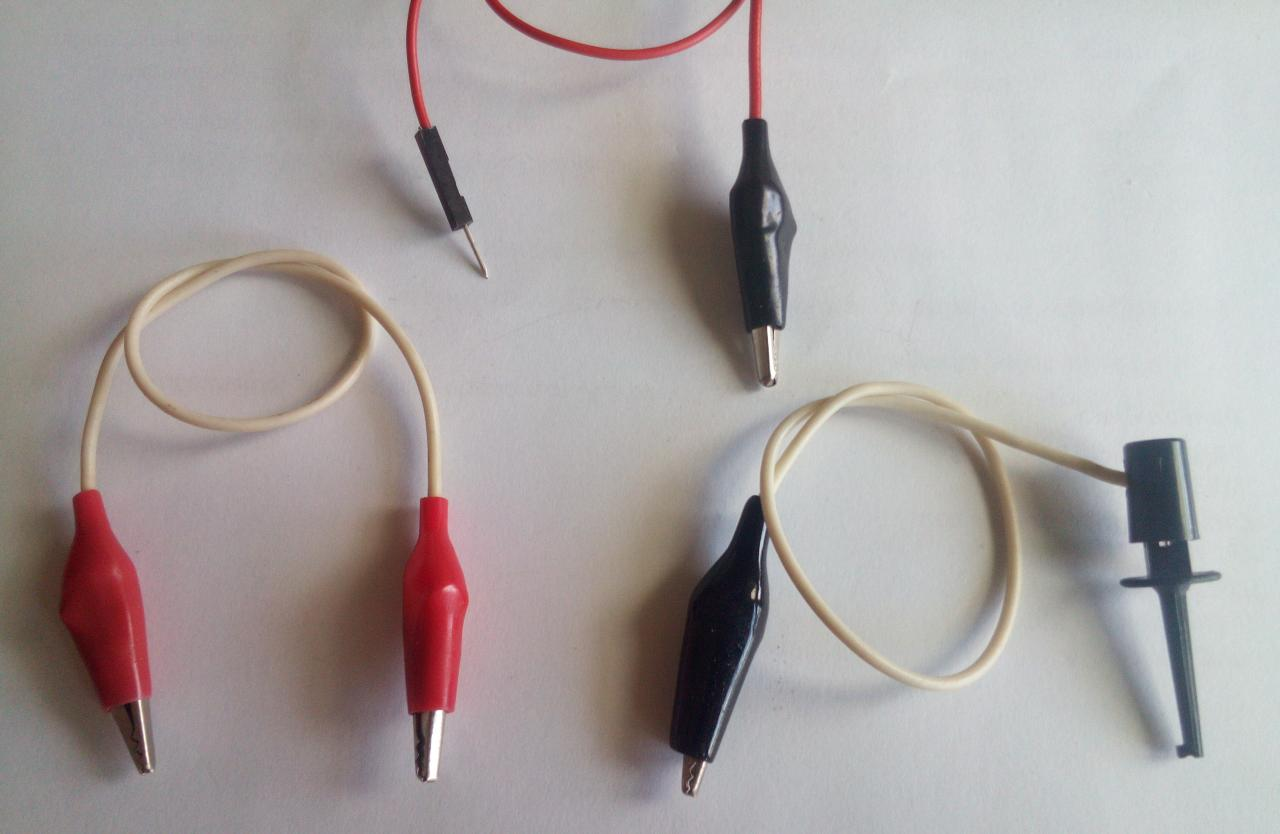
\includegraphics[height=5.3cm]{warsztat_elektroniczny/krokodylki}\footnotesize
		\\od lewej: przewód krokodylek - krokodylek (biało-czerwony), krokodylek - pin męski (czerwono-czarny), krokodylek - chwytak (biało-czarny)
	}
\hspace{\stretch{2}}
\vspace{12pt}

Koszt płytki prototypowej, zestawu kabelków i śrubokręta to około 20PLN.

% Copyright (c) 2017-2020 Matematyka dla Ciekawych Świata (http://ciekawi.icm.edu.pl/)
% Copyright (c) 2017-2020 Robert Ryszard Paciorek <rrp@opcode.eu.org>
% 
% MIT License
% 
% Permission is hereby granted, free of charge, to any person obtaining a copy
% of this software and associated documentation files (the "Software"), to deal
% in the Software without restriction, including without limitation the rights
% to use, copy, modify, merge, publish, distribute, sublicense, and/or sell
% copies of the Software, and to permit persons to whom the Software is
% furnished to do so, subject to the following conditions:
% 
% The above copyright notice and this permission notice shall be included in all
% copies or substantial portions of the Software.
% 
% THE SOFTWARE IS PROVIDED "AS IS", WITHOUT WARRANTY OF ANY KIND, EXPRESS OR
% IMPLIED, INCLUDING BUT NOT LIMITED TO THE WARRANTIES OF MERCHANTABILITY,
% FITNESS FOR A PARTICULAR PURPOSE AND NONINFRINGEMENT. IN NO EVENT SHALL THE
% AUTHORS OR COPYRIGHT HOLDERS BE LIABLE FOR ANY CLAIM, DAMAGES OR OTHER
% LIABILITY, WHETHER IN AN ACTION OF CONTRACT, TORT OR OTHERWISE, ARISING FROM,
% OUT OF OR IN CONNECTION WITH THE SOFTWARE OR THE USE OR OTHER DEALINGS IN THE
% SOFTWARE.

\subsection{Mikrokontroler - Moduł STM32}

\parbox[c]{0.55\textwidth}{
	W ramach zajęć będziemy uczyć się podstaw programowania mikrokontrolerów w oparciu o mikrokontroler STM32F103C8.
	W tym celu potrzebne będą nam płytka zawierająca mikrokontroler wraz niezbędnymi peryferiami - będziemy używać tzw. modułu „blue-pill” pokazanego na zdjęciu obok. Cena od około 11.5PLN.
}
\hspace{\stretch{1}}
\parbox[c]{0.43\textwidth}{
	\begin{flushright} 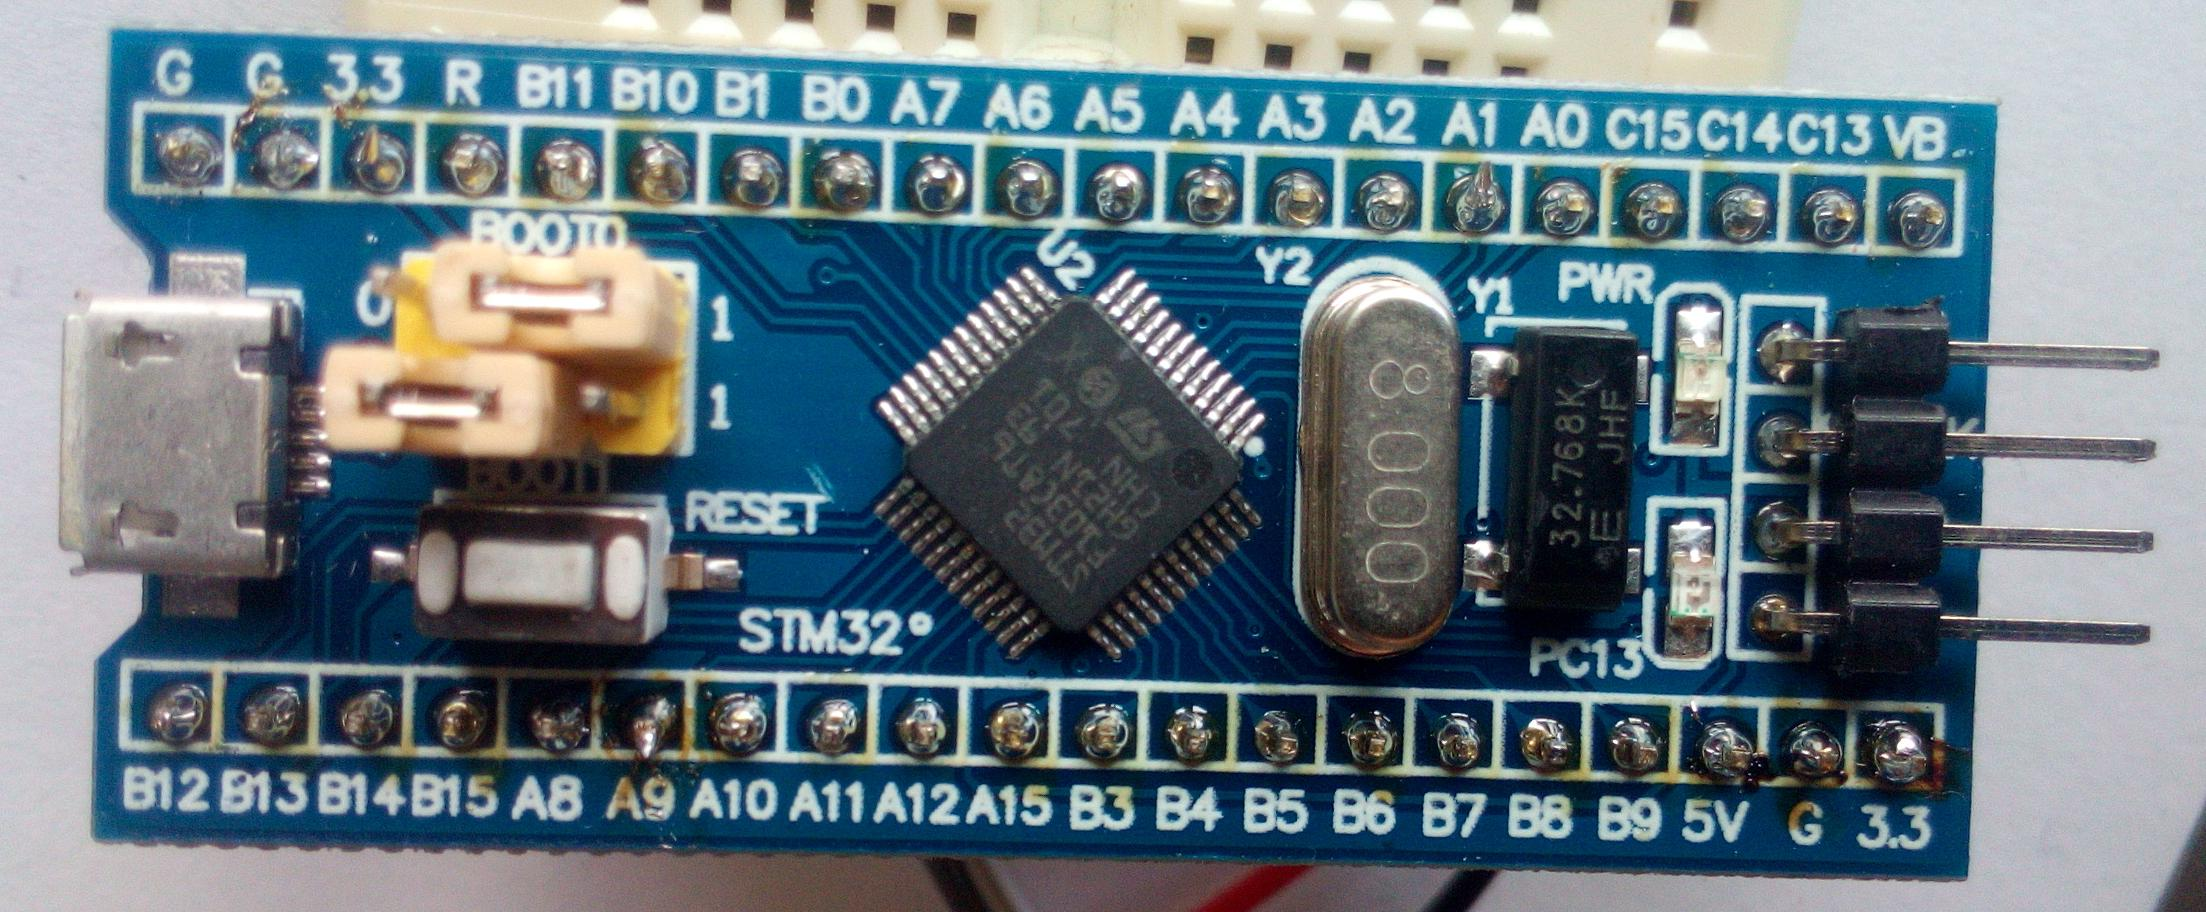
\includegraphics[height=3.3cm]{warsztat_elektroniczny/blue-pill} \end{flushright}
}


\subsection{Programator do STM32 – Konwerter USB-UART}

Do programowania użyjemy portu szerowego naszego mikrokontrolera, w celu połączenia się z nim potrzebna będzie przejściówka USB-UART. Zasadniczo dowlna tego typu przejściówka (mająca napięcia logiczne na poziomie 3.3V, czyli \textbf{nie} przejściówka typu RS232) będzie OK. Poniżej dwie przetestowane propozycje do wyboru.

\subsubsection{Moduł z układem PL2303HX}
\parbox[c]{0.55\textwidth}{
	\begin{itemize}
		\wada moduł ma wyprowadzone jedynie linie RxD i TxD
		\wada moduł do wygodnego używania wymaga przedłużacza USB
		\info od 3.5PLN
	\end{itemize}
}
\hspace{\stretch{1}}
\parbox[c]{0.43\textwidth}{
	\begin{flushright} 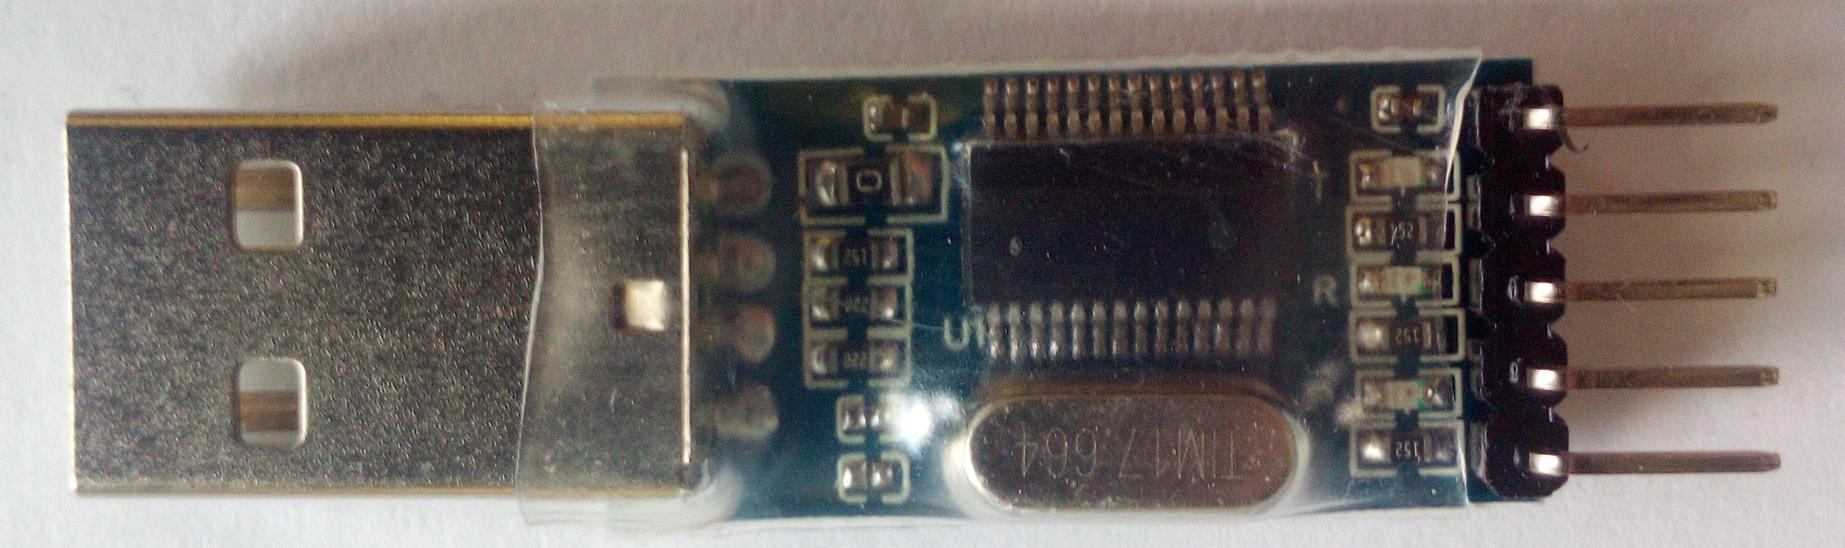
\includegraphics[height=2.3cm]{warsztat_elektroniczny/usb-uart1} \end{flushright}
}

\subsubsection{Moduł z układem FTDI FT232RL}
\parbox[c]{0.65\textwidth}{
	\begin{itemize}
		\zaleta moduł ma wyprowadzone na bocznych wszystkie linie portu szeregowego, co prawda nam nie będzie to potrzebne, ale może się przydać w innych zastosowaniach (np. programowanie układów ESP)
		\wada moduł wymaga kabla mini-usb
		\info od 10PLN
	\end{itemize}
}
\hspace{\stretch{1}}
\parbox[c]{0.33\textwidth}{
	\begin{flushright} 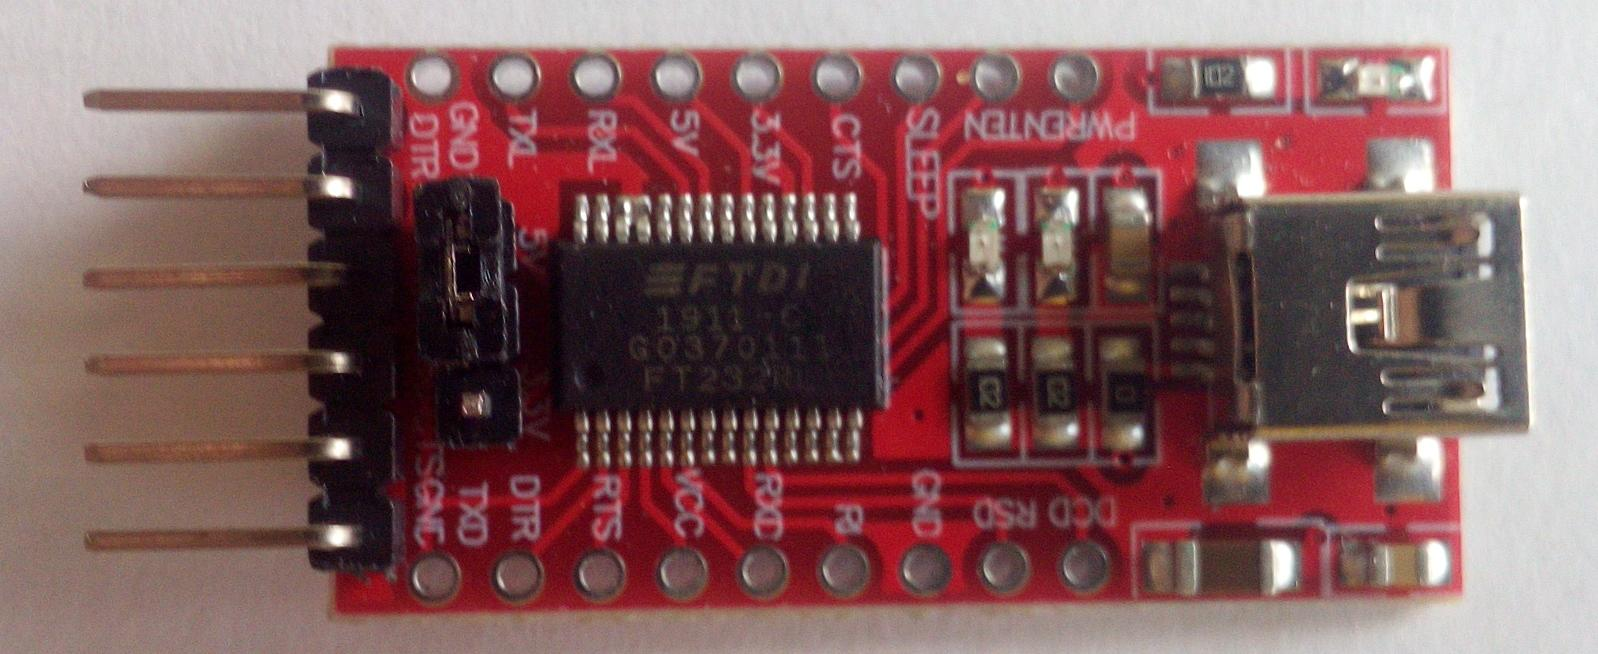
\includegraphics[height=2.3cm]{warsztat_elektroniczny/usb-uart2} \end{flushright}
}

\input{booklets-sections/warsztat/15-zakupy-podzespoły.tex}
% Copyright (c) 2017-2020 Matematyka dla Ciekawych Świata (http://ciekawi.icm.edu.pl/)
% Copyright (c) 2017-2020 Robert Ryszard Paciorek <rrp@opcode.eu.org>
% 
% MIT License
% 
% Permission is hereby granted, free of charge, to any person obtaining a copy
% of this software and associated documentation files (the "Software"), to deal
% in the Software without restriction, including without limitation the rights
% to use, copy, modify, merge, publish, distribute, sublicense, and/or sell
% copies of the Software, and to permit persons to whom the Software is
% furnished to do so, subject to the following conditions:
% 
% The above copyright notice and this permission notice shall be included in all
% copies or substantial portions of the Software.
% 
% THE SOFTWARE IS PROVIDED "AS IS", WITHOUT WARRANTY OF ANY KIND, EXPRESS OR
% IMPLIED, INCLUDING BUT NOT LIMITED TO THE WARRANTIES OF MERCHANTABILITY,
% FITNESS FOR A PARTICULAR PURPOSE AND NONINFRINGEMENT. IN NO EVENT SHALL THE
% AUTHORS OR COPYRIGHT HOLDERS BE LIABLE FOR ANY CLAIM, DAMAGES OR OTHER
% LIABILITY, WHETHER IN AN ACTION OF CONTRACT, TORT OR OTHERWISE, ARISING FROM,
% OUT OF OR IN CONNECTION WITH THE SOFTWARE OR THE USE OR OTHER DEALINGS IN THE
% SOFTWARE.

\subsection{Inne}
Jeżeli kupiony moduł STM32 nie ma przylutowanych pinów po bokach (a na ogół nie ma), będzie potrzebna także lutownica z cyną i kalafonią. Koszt od 16PLN.

Przydać mogą się także małe obcążki boczne, szczypce, czy też jakiś nożyk.

Oczywiście do programowania mikrokotrolera będzie potrzebny także działający komputer z portem USB i system Linux (da się na innych systemach operacyjnych, ale to na Linuxie będzie oparte nasze środowisko do tworzenia programów dla STM32), jednak zakładamy że jakiś już masz {\Symbola 😄}.


% Copyright (c) 2017-2020 Matematyka dla Ciekawych Świata (http://ciekawi.icm.edu.pl/)
% Copyright (c) 2017-2020 Robert Ryszard Paciorek <rrp@opcode.eu.org>
% Copyright (c) 2020 Krzysztof Lasocki <krz.lasocki@gmail.com>
% 
% MIT License
% 
% Permission is hereby granted, free of charge, to any person obtaining a copy
% of this software and associated documentation files (the "Software"), to deal
% in the Software without restriction, including without limitation the rights
% to use, copy, modify, merge, publish, distribute, sublicense, and/or sell
% copies of the Software, and to permit persons to whom the Software is
% furnished to do so, subject to the following conditions:
% 
% The above copyright notice and this permission notice shall be included in all
% copies or substantial portions of the Software.
% 
% THE SOFTWARE IS PROVIDED "AS IS", WITHOUT WARRANTY OF ANY KIND, EXPRESS OR
% IMPLIED, INCLUDING BUT NOT LIMITED TO THE WARRANTIES OF MERCHANTABILITY,
% FITNESS FOR A PARTICULAR PURPOSE AND NONINFRINGEMENT. IN NO EVENT SHALL THE
% AUTHORS OR COPYRIGHT HOLDERS BE LIABLE FOR ANY CLAIM, DAMAGES OR OTHER
% LIABILITY, WHETHER IN AN ACTION OF CONTRACT, TORT OR OTHERWISE, ARISING FROM,
% OUT OF OR IN CONNECTION WITH THE SOFTWARE OR THE USE OR OTHER DEALINGS IN THE
% SOFTWARE.

\section{Obsługa multimetru}

Multimetr (zwany też miernikiem) to podstawowy przyrząd pomiarowy każdego elektronika. Zgodnie z nazwą posiada wiele funkcji pomiarowych.
Najczęściej są to woltomierz (do pomiaru napięcia stałego \textbf{V$\mathdirectcurrent$} i zmiennego \textbf{V$\sim$}),
amperomierz (do pomiaru natężenia prądu stałego \textbf{A$\mathdirectcurrent$} i zmiennego \textbf{A$\sim$}, potocznie zwanego prądem)
oraz omomierz (do pomiaru rezystancji, \textbf{$\Omega$}). Często multimetr posiada także funkcje:
\begin{itemize}
\item \textbf{Test połączeń} (\textit{continuity mode}), oznaczany symbolem fali dźwiękowej (lub nuty), służy do sprawdzania połączeń elektrycznych.
  Miernik wydaje dźwięk jeśli między sondami pomiarowymi (przewodami) jest połączenie.
\item \textbf{Pomiar diod} (\textit{diode check}), oznaczony symbolem diody \esymbol{diode}, służy do sprawdzania diod i innych elementów półprzewodnikowych.
  Wyświetla spadek napięcia na testowanym złączu półprzewodnikowym.
\item \textbf{Test tranzystorów} (pomiar h\textsubscript{FE}), służący do pomiaru wzmocnienia tranzystora. Najczęściej posiada oddzielne gniazdo
  na mierniku.
\item \textbf{Pomiar pojemności}, oznaczany symbolem \esymbol{capacitor} służy do pomiarów pojemności kondensatorów
\item \textbf{Pomiar temperatury}, ocznaczany symbolem \textbf{$^{\circ}$C}, najczęściej za pomocą termopary (dołączana do miernika).
\end{itemize}

Multimetr zachowuje się tak jak przyrząd pomiarowy, którego funkcjonalność jest aktualnie wybrana. Oznacza to że należy go podłączać
tak samo, jak odpowiednie przyrządy pomiarowe. 

\subsection{Połączenie miernika}
W zależności od modelu, multimetr może posiadać od dwóch do czterech gniazd na przewody. Są to:
\begin{itemize}
\item Masa, oznaczana \textbf{COM} (od słowa \textit{common}). Tutaj podłącza się czarny przewód
\item Wejście pomiarowe dla woltomierza, ozn. symbolem \textbf{V}. Często także jest to wejście omomierza, oznaczone \textbf{$\Omega$},
  oraz testu diod (ozn. symbolem diody \esymbol{diode})
\item Wejście miliamperomierza, oznaczone symbolem \textbf{mA}. Jeżeli Twój miernik posiada trzy wejścia, to najczęściej jest ono
  tym samym wejściem, co wejście woltomierza.
\item Wejście amperomierza, oznaczone symbolem \textbf{A}. Najczęściej również jest obok niego podany maksymalny dopuszczalny prąd
  oraz czas pomiaru.
\end{itemize}

\begin{Ramka}{}\begin{center}
  {\noindent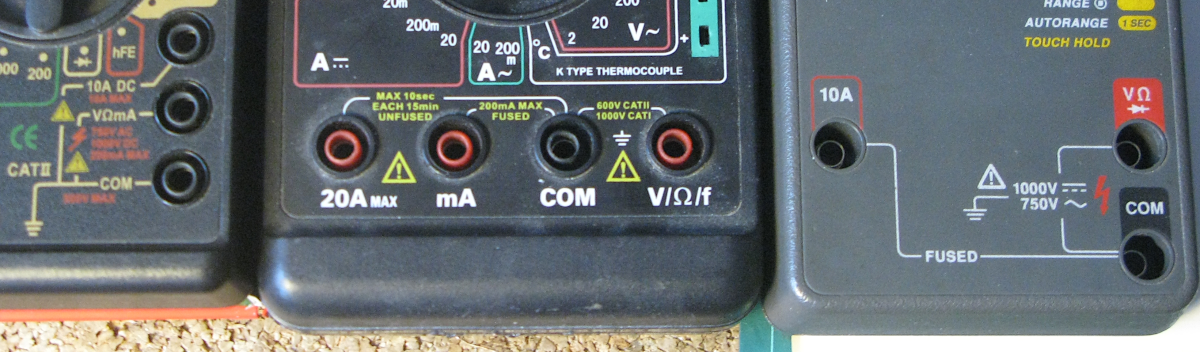
\includegraphics[width=0.99\textwidth,clip=true]{warsztat_elektroniczny/dmm_terminals}}\\
  \small
  Wejścia trzech różnych multimetrów. Pomiędzy wejściami zaznaczone są maksymalne wartości napięcia lub natężenia i informacja o zabezpieczeniach  (``FUSED'') bądź ich braku (``UNFUSED'').\\
  Od lewej: typowy model z trzema wejściami, model z czterema wejściami, model z trzema wejściami (bez miliamperomierza)
\end{center}\end{Ramka}

Przy wyborze multimetru należy zwrócić uwagę na jego wejścia. Modele z czterema wejściami są preferowane (zapewnia to izolację funkcji woltomierza
od amperomierza). Przyrząd musi być też opisany jako ``FUSED'', czyli posiadać bezpiecznik na zakresie miliamperomierza (oraz opcjonalnie,
także amperomierza). Pozwoli to uniknąć uszkodzenia multimetru w wypadku przekroczenia dopuszczalnego natężenia prądu.

\subsection{Woltomierz}
Woltomierz to przyrząd służący do pomiaru napięcia elektrycznego między dwoma punktami. Z tego powodu
\textbf{woltomierz podłączamy równolegle} do elementu, który badamy, lub między dwoma punktami w układzie. Opór woltomierza jest możliwie duży (rzeczywiste
woltomierze mają opór około 1-10 M$\Omega$, woltomierz idealny ma opór nieskoczenie wysoki).

\subsection{Amperomierz}
Amperomierz (tudzież miliamperomierz) służy do pomiaru prądu płynącego w gałęzi obwodu. Z tego powodu
\textbf{amperomierz podłączamy szeregowo} z innymi elementami obwodu. Opór amperomierza jest możliwie mały (idealny amperomierz
ma nieskończenie niski opór).
\\

Podłączenie amperomierza równolegle powoduje zwarcie. Nie należy więc odkładać miernika ustawionego na zakres amperów, szczególnie
w przypadku modeli, które używają tego samego gniazda do pomiaru oporności lub napięcia. Skutki pomyłki mogą być fatalne dla
urządzenia - bezpiecznik się spali.

\subsection{Omomierz}
Omomierz jest przyrządem służącym do pomiaru oporności. Jego zasada działania jest dosyć prosta. Składa się on ze źrodła małego napięcia, które pojawia się na końcówkach przewodów pomiarowych. Gdy przyłożymy sondy do elementu mierzonego, omomierz zmierzy jaki prąd płynie przez element testowany i wyświetli jego opór.
\\

Omomierz w praktyce służy tylko do pomiarów oporników. Trzeba pamiętać o tym, że jeżeli mierzymy element umieszczony w układzie,
to jego oporność będzie zawsze niższa od oczekiwanej. Taki opornik jest połączony równolegle z innymi elementami obwodu o
nieznanym oporze, skąd wynika błąd pomiaru.
Zasadniczo nie wykonuje się za jego pomocą pomiarów oporników we włączonych układach.
\\

Przy pomiarach większych oporników (ponad 100k$\Omega$) należy uważać aby nie dotykać palcami końcówek sond, ponieważ opór Twojego ciała
zaniży pomiar. Lepiej jest położyć opornik na stole i przycisnąć jego nóżki za pomocą końcówek sond.


\subsection{Inne funkcje multimetrów}
Oprócz podstawowych funkcji (pomiaru napięcia, natężenia i oporu)\footnotemark, większość nowoczesnych multimetrów posiada także funkcje pomiaru diod oraz tranzystorów.
\\

Funkcja pomiaru diod jest najczęściej oznaczona symbolem diody półprzewodnikowej (\esymbol{diode}) i korzysta z tej samej pary złącz, co woltomierz i omomierz.
Aby zmierzyć spadek napięcia na diodzie należy dotknąć sondą podłączoną do masy (COM) do katody, a sondą dodatnią do anody. Miernik wyświetli
spadek napęcia na złączu diody. Jeżeli miernik wskazuje wynik poza skalą, może to oznaczać, że polaryzacja diody jest odwrotna (sondy są przyłożone na odwrót).
Może też okazać się, że spadek napięcia na jej złączu jest większy niż zakres pomiaru (który najczęściej wynosi do 2V).
\\

\footnotetext{Mierniki, które posiadają tylko te trzy funkcje nazywane są po angielsku VOM (Volt-ohm-milliammeter). Najczęściej są to mierniki
  analogowe.}

\begin{wrapfigure}{r}{0.19\textwidth}
  \begin{center}
    \vspace{-25pt}
    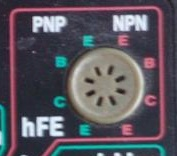
\includegraphics[width=0.17\textwidth]{warsztat_elektroniczny/multimetr_hfe.jpg}
    \vspace{-20pt}
  \end{center}
\end{wrapfigure}

Funkcja pomiaru współczynnika wzmocnienia tranzystora bipolarnego jest z reguły oznaczana \textbf{hFE} (od symbolu $\text{h}_{FE}$ stosowanego do
oznaczenia tej wartości)\footnote{Czasami oznaczanego też jako $\beta$, beta.}. Pomiar tranzystora za pomocą multimetru polega na umieszczeniu jego nóżek w \textbf{odpowiedni sposób} w gnieździe pomiarowym
w multimetrze. Jego emiter, baza oraz kolektor (oznaczane \textbf{E}, \textbf{B} i \textbf{C} odpowiednio) muszą trafić w
otwory w odpowiedniej połowie gniazda (\textbf{PNP} oraz \textbf{NPN} zależnie od typu tranzystora). Trzeba go obrócić tak, żeby emiter trafił do \textbf{E}, baza do \textbf{B} a kolektor do \textbf{C}.
Gniazdo jest tak skonstruowane, że pasują do niego tranzystory o dowolnej kolejności wyprowadzeń. Kolejność dla Twojego tranzystora jest opisana w jego karcie katalogowej.
Po umieszczeniu tranzystora w gnieździe, na ekranie miernika pojawia się wartość jego współczynnika wzmocnienia $\text{h}_{FE}$.
\\

Niektóre mierniki posiadają także funkcje pomiaru pojemności elektrycznej kondensatora. W zależności od konstrukcji połączenie testowanego
kondensatora odbywa się poprzez umieszczenie go w specjalnym gnieździe na obudowie miernika albo przez podłączenie sond do wyprowadzeń kondensatora. Należy pamiętać
o tym, że trzeba ustawić zakres w podobny sposób jak przy innych pomiarach. Uwaga - \textbf{nie należy mierzyć pojemności naładowanych
  kondensatorów}. Funkcja pomiaru pojemności przydaje się przy sprawdzaniu kondensatorów ceramicznych lub foliowych o pojemnościach od kilku nF do kilkudziesięciu uF. Na kondensatorach elektrolitycznych lub tantalowych (o większych pojemnościach) wartość
pojemności jest z reguły napisana na obudowie. Należy także wybrać kondensator, którego maksymalne dopuszczalne napięcie (też napisane na obudowie)
jest wyższe niż największe możliwe napięcie mogące na nim wystąpić w układzie.

\begin{ProTip}{\normalfont{\strong{Uwaga}}}
  Kondensatory elektrolityczne oraz tantalowe są elementami \textbf{spolaryzowanymi}. Podłączając je, należy o tym pamiętać i podłączać je
  tylko zgodnie z polaryzacją - biegun ujemny do punktu o niższym napięciu, a biegun dodatni do punktu o wyższym napięciu. Na tych kondensatorach jeden
  z biegunów (najczęściej ujemny) jest zaznaczony na obudowie.
  
  \textbf{Uwaga:} Niewłaściwe podłączenie kondensatora może doprowadzić do jego eksplozji.
  Dla własnego bezpieczeństwa nie rób tego – jeżeli jesteś ciekawy jak to wygląda obejrzyj filmik w Internecie.
  Pamiętaj o tym także montując kondensatory w swoich konstrukcjach.
\end{ProTip}

Oprócz opisanych wyżej funkcji, niektóre multimetry mogą mieć także funkcje pomiaru temperatury (poprzez \textbf{termoparę}
lub \textbf{termistor} podłączane do
specjalnego złącza na mierniku) oraz pomiar częstotliwości.

\subsection{Dokonywanie pomiarów}

Zależnie od wielkości fizycznej, którą chcemy zmierzyć, po stroni emiernika, czerwony (dodatni) przewód musi być podłączony do odpowiadającego
mu gniazda. Czarny przewód (ujemny, masa) należy zawsze podłączyć do gniazda \textbf{COM}. Miernik ustawiamy na pomiar danej
wielkości.
\\

Przy wykonywaniu pomiaru nieznanej wartości należy rozpocząć od największego zakresu miernika i stopniowo zmniejszać zakres aż
otrzymamy najdokładniejszy wynik. W przypadku gdy mierzona wartość przekracza aktualny zakres, miernik to zasygnalizuje, najczęściej
wyświetlając ``\textbf{1}'' (po lewej stronie ekranu), lub ``\textbf{OL}'' (\emph{overload}). Oba znaki oznaczają to samo, czyli wartość powyżej zakresu. W takiej sytuacji trzeba przełączyć zakres na większy.
\\

Przy pomiarze \textbf{napięcia} w danym punkcie układu, najczęściej masę miernika (czarną sondę)
podłączamy do masy układu. Drugą sondę (czerwoną) podłączamy do mierzonego punktu. Jeśli chcemy zmierzyć napięcie na jakimś elemencie (np. oporniku),
masą miernika dotykamy do punktu, w którym oczekujemy niższego napięcia, a czerwoną sondą do punktu, w którym oczekujemy
wyższego napięcia. Jeżeli podłączymy sondy odwrotnie, po prostu dostaniemy wynik z przeciwnym znakiem. Woltomierz należy podłączać równolegle.
\\

Przy pomiarze \textbf{natężenia} w danej gałęzi układu należy zachować szczególną ostrożność. Podobnie jak wyżej, zaczynamy pomiar na największym
zakresie miernika. W przeciwieństwie do woltomierza, amperomierz należy podłączyć szeregowo. Ponieważ opór wewnętrzny amperomierza jest bardzo
niski (<1~$\Omega$), trzeba uważać, aby nie zrobić zwarcia.
\\

Pomiaru \textbf{oporności} dokonujemy dotykając końcówkami sond pomiarowych końcówek opornika (lub innego elementu). Dla oporników kolejność przewodów nie ma znaczenia
(opór jest identyczny niezależnie od kierunku płynięcia prądu).
\\

Test połączenia służy do sprawdzania połączeń w układach. Przy wyłączonym zasilaniu dotykamy sondami do punktów, pomiędzy którymi chcemy
sprawdzić połączenie. Jeżeli punkty są połączone, to miernik zasygnalizuje to brzęczykiem. Ta funkcja jest szczególnie przydatna przy sprawdzaniu
prototypów na płytkach stykowych, lub przy sprawdzaniu prawidłowości połączeń w urządzeniu, które diagnozujemy. Jeżeli Twój
multimetr nie ma tej funkcji, to możesz użyć omomierza (bezpośrednie połączenie ma znikomy opór, maksymalnie kilka~$\Omega$).
\\

Tester diod (i innych elementów półprzewodnikowych) pozwala sprawdzić polaryzację złącza półprzewodnikowego w elemencie. W tym celu dotykamy
sondami do obu końców testowanego elementu. Jeżeli ``trafiliśmy'' z polaryzacją sond (podłączyliśmy czarną sondę, COM, do katody, a czerwoną
dodatnią, do anody), to miernik powinien pokazać spadek napięcia na złączu.
W przeciwnym razie pokaże przekroczenie zakresu. Z reguły zakres spadków napięć jakie można w tym trybie zmierzyć jest poniżej 2V, więc
większość diod LED pokaże spadek napięcia poza skalą (niektóre diody LED mogą się bardzo słabo świecić podczas pomiaru jeśli polaryzacja
sond jest prawidłowa).
\\

W niektórych multimetrach test diody jest wspólny z testem połączeń. W takim wypadku, w trybie testu multimetr sygnalizuje
buzzerem sytuację, gdy spadek napięcia jest odpowiednio mały. Oznacza to, że mierzone punkty są ze sobą zwarte
(lub połączone bardzo małym oporem).\\

\begin{ProTip}{\normalfont{\strong{Wskazówka}}}
  W zmontowanym i zasilonym układzie należy dokonywać tylko pomiarów woltomierzem.
  Amperomierz włącza się w szeregowo w badany układ, zatem jego użycie wymaga modyfikacji układu, chyba że układ przewiduje możliwość takiego pomiaru.
  
  Omomierz i pomiar pojemności używa się do pomiarów elementów poza układem,
  jednak pomiar ciągłości (rzadziej oporności) może być wykonywany na wyłączonym układzie celem ustalenia dlaczego ten nie działa.
  Należy wtedy pamiętać o tym, że pomiary omomierzem będą zaniżone z  powodu obecności innych oporów w układzie.
\end{ProTip}

% Copyright (c) 2017-2020 Matematyka dla Ciekawych Świata (http://ciekawi.icm.edu.pl/)
% Copyright (c) 2017-2020 Robert Ryszard Paciorek <rrp@opcode.eu.org>
% Copyright (c) 2020 Krzysztof Lasocki <krz.lasocki@gmail.com>
% 
% MIT License
% 
% Permission is hereby granted, free of charge, to any person obtaining a copy
% of this software and associated documentation files (the "Software"), to deal
% in the Software without restriction, including without limitation the rights
% to use, copy, modify, merge, publish, distribute, sublicense, and/or sell
% copies of the Software, and to permit persons to whom the Software is
% furnished to do so, subject to the following conditions:
% 
% The above copyright notice and this permission notice shall be included in all
% copies or substantial portions of the Software.
% 
% THE SOFTWARE IS PROVIDED "AS IS", WITHOUT WARRANTY OF ANY KIND, EXPRESS OR
% IMPLIED, INCLUDING BUT NOT LIMITED TO THE WARRANTIES OF MERCHANTABILITY,
% FITNESS FOR A PARTICULAR PURPOSE AND NONINFRINGEMENT. IN NO EVENT SHALL THE
% AUTHORS OR COPYRIGHT HOLDERS BE LIABLE FOR ANY CLAIM, DAMAGES OR OTHER
% LIABILITY, WHETHER IN AN ACTION OF CONTRACT, TORT OR OTHERWISE, ARISING FROM,
% OUT OF OR IN CONNECTION WITH THE SOFTWARE OR THE USE OR OTHER DEALINGS IN THE
% SOFTWARE.

\section{Przetwornica zasilająca}

Przetwornica z regulacją napięcia i ograniczenia prądowego będzie pełniła funkcję (stosunkowo taniego i przenośnego) zasilacza laboratoryjnego.

\subsection{Uruchomienie}
\subsubsection{Zasilanie przetwornicy}

\begin{wrapfigure}{r}{0.35\textwidth}
  \begin{center}
    \vspace{-40pt}
    \includegraphics[width=0.33\textwidth]{warsztat_elektroniczny/przewody_zasilające.jpg}
    \vspace{-40pt}
  \end{center}
\end{wrapfigure}


Nasza przetwornica może być zasilona z baterii 9V lub zasilacza wtyczkowego 12V DC.
Zarówno gniazdo baterii jak i zasilacz może być wyposażone we wtyk DC 2.5/5.5 lub 2.1/5.5 (taki jak widoczny na zdjęciu obok) lub bezpośrednio wyprowadzone przewodu.
W przypadku zastosowania wtyku DC będzie możliwe łatwe odłączanie zasilania od przetwornicy. Jednak konieczne jest wtedy użycie także odpowiedniego gniazda DC.

\begin{ProTip}{\normalfont{\strong{Uwaga}}}
  \textbf{Niektóre przetwornice nie są odporne na niepoprawną polaryzację wejścia. Odwrotne podłączenie napięcia do wejścia takiej przetwornicy doprowadzi do jej zniszczenia. Dlatego odłącz przetwornicę od kabli zasilających zanim sprawdzisz ich polaryzację.}
\end{ProTip}

\vspace{13pt}\noindent
Niezależnie od tego, czy do zasilania przetwornicy używamy baterii, czy zasilacza wtyczkowego, musimy~\textbf{sprawdzić
  polaryzację przewodów, które będziemy podłączać do przetwornicy}. 
\\

\noindent W tym celu:
\begin{itemize}
	\item \textbf{odłączamy przewody zasilające od przetwornicy}.
	\item wkładamy wtyk DC do gniazda DC zasilacza.
	\item włączamy multimetr i nastawiamy go na pomiar napięcia stałego (DC) w zakresie do 20V.
	\item dbając o to, aby przewody zasilające nie zetknęły się ze sobą (aby uniknąć zwarcia) podłączamy zasilanie, czyli wkładamy zasilacz wtyczkowy do gniazdka lub podłączamy baterię do złącza baterii.
	\item dokonujemy pomiaru napięcia na przewodach zasilających, podłączając czerwoną sondę (dodatnią) do czerwonego przewodu, a masę (czarną sondę) do czarnego przewodu.
        \item Multimetr powinien wskazać dodatnie napięcie. Jeżeli wskazuje ujemne, to znaczy, że polaryzacja naszego przewodu~zasilającego jest odwrotna. W takiej sytuacji \textbf{czerwony} przewód od zasilacza (lub baterii) jest \textbf{ujemny} a \textbf{czarny} jest \textbf{dodatni}. Jeśli multimetr wskazuje napięcie dodatnie, oznacza to, że kolory przewodów są zgodne z polaryzacją. 
	\item zapisujemy jaki kolor przewodu odpowiada masie, a jaki biegunowi dodatniemu.
	\item \textbf{wyłączamy zasilanie} – wyjmujemy wtyk DC z gniazdka DC, odłączamy baterię od złącza lub wyjmujemy zasilacz wtyczkowy z gniazdka.
\end{itemize}
Teraz możemy przykręcić przewody zasilające do naszej przetwornicy. Należy zwrócić szczególną uwagę aby podłączyć je do zacisków wejściowych (oznaczonych jako \texttt{IN}) z zachowaniem ustalonej przez nas polaryzacji:
\begin{itemize}
	\item przewód na którym mieliśmy masę (biegun ujemny) podłączamy do IN- / GND
	\item przewód na którym mieliśmy biegun dodatni podłączamy do IN+
\end{itemize}

\begin{wrapfigure}{r}{0.4\textwidth}
  \begin{center}
    \vspace{-30pt}
    \includegraphics[width=0.4\textwidth]{warsztat_elektroniczny/moduł_XL4015_LCD_2.jpg}
    \vspace{-50pt}
  \end{center}
\end{wrapfigure}

\subsubsection{Regulacja przetwornicy}

W celu sprawdzenia działania przetwornicy:
\begin{itemize}
	\item do wyjścia przetwornicy podłączamy multimetr nastawiony na zakres pomiaru napięcia stałego (DC) do 20V.
	\item włączamy zasilanie przetwornicy – wkładamy wtyk DC do gniazdka DC, podłączamy baterię od złącza lub wkładamy zasilacz wtyczkowy z gniazdka.
	\item multimetr wyświetla napięcie na wyjściu przetwornicy. Jeżeli nasza przetwornica posiada wbudowany woltomierz to wskazania obu przyrządów powinny być podobne (mogą się różnić o ułamkowe części wolta).
\end{itemize}
\vspace*{\baselineskip}


Przetwornica posiada dwa potencjometry – jeden służy do regulacji napięcia, a drugi do regulacji ograniczenia prądowego. Zazwyczaj są podpisane, ale jeżeli nie są, to możemy łatwo ustalić, który za co odpowiada.
W tym celu, przy pomocy odpowiedniego wkrętaka, obróć śrubkę regulacyjną potencjometru od napięcia i zobacz jak wpływa to na napięcie wyjściowe.

Nastaw napięcie wyjściowe na 5V. Drugi potencjometr odpowiedzialny jest za regulację prądu. Ustaw go w okolicy wartości minimalnej:
\begin{itemize}
	\item pokręć nim aż do oporu lub kliknięcia w tę samą stronę, która odpowiadała za zmniejszanie napięcia w potencjometrze od regulacji napięcia.
	\item zrób pół obrotu w przeciwną stronę.
\end{itemize}
Następnie:
\begin{itemize}
	\item odłącz multimetr od wyjścia przetwornicy, nastaw na pomiar prądu do 10A lub 20A i podłącz sondy do odpowiednich gniazd w mierniku.
	\item przytknij na krótko (około 1 – 2 sekund) sondy do zacisków wyjściowych i zaobserwuj wskazanie multimetru.
\end{itemize}
Jeżeli wskazanie było duże (około ampera lub kilku) obrócić potencjometr odpowiedzialny za regulację prądu w przeciwnym kierunku i ponów procedurę pomiaru.
Jeżeli było ono poniżej 0.2A przestaw multimetr na zakres 200mA, przełóż sondy do odpowiednich gniazd i ponownie wykonaj pomiar.

Nastaw ograniczenie prądowe na około 40mA.

% Copyright (c) 2017-2020 Matematyka dla Ciekawych Świata (http://ciekawi.icm.edu.pl/)
% Copyright (c) 2017-2020 Robert Ryszard Paciorek <rrp@opcode.eu.org>
% Copyright (c) 2020 Krzysztof Lasocki <krz.lasocki@gmail.com>
% 
% MIT License
% 
% Permission is hereby granted, free of charge, to any person obtaining a copy
% of this software and associated documentation files (the "Software"), to deal
% in the Software without restriction, including without limitation the rights
% to use, copy, modify, merge, publish, distribute, sublicense, and/or sell
% copies of the Software, and to permit persons to whom the Software is
% furnished to do so, subject to the following conditions:
% 
% The above copyright notice and this permission notice shall be included in all
% copies or substantial portions of the Software.
% 
% THE SOFTWARE IS PROVIDED "AS IS", WITHOUT WARRANTY OF ANY KIND, EXPRESS OR
% IMPLIED, INCLUDING BUT NOT LIMITED TO THE WARRANTIES OF MERCHANTABILITY,
% FITNESS FOR A PARTICULAR PURPOSE AND NONINFRINGEMENT. IN NO EVENT SHALL THE
% AUTHORS OR COPYRIGHT HOLDERS BE LIABLE FOR ANY CLAIM, DAMAGES OR OTHER
% LIABILITY, WHETHER IN AN ACTION OF CONTRACT, TORT OR OTHERWISE, ARISING FROM,
% OUT OF OR IN CONNECTION WITH THE SOFTWARE OR THE USE OR OTHER DEALINGS IN THE
% SOFTWARE.

\section{Przygotowanie mikrokontrolera STM32}

Bardzo możliwe, że Twój mikrokontroler nie będzie miał przylutowanych pinów do połączenia z płytką stykową.
W takim wypadku będziesz musiał/musiała użyć lutownicy, aby je przylutować.\\

\begin{ProTip}{\normalfont{\strong{Ostrożnie}}}
  Podczas pracy, grot (metalowa końcówka) lutownicy jest rozgrzany do 200-400 stopni Celsjusza. Zachowaj ostrożność
  podczas jej używania. Zapamiętaj:
  \begin{itemize}
  \item Zawsze odkładaj lutownicę do stojaka. Nigdy nie kładź jej luzem na stole.
  \item Nigdy nie łap za metalowy koniec lutownicy.
  \item Nie wolno łapać spadającej lutownicy. Nie martw się, zawszę można kupić nową.
  \item Grot lutownicy jest gorący przez jakiś czas po wyłączeniu.
  \item Nie zostawiaj włączonej lutownicy bez opieki.
  \item \textbf{Przed lutowaniem musisz odłączyć układ (lub urządzenie) od zasilania}.
  \end{itemize}
\end{ProTip}

Do lutowania drobnej elektroniki (takiej jak mikrokontrolery i układy scalone) najepsza jest precyzyjna lutownica o małej mocy (do 30W),
z regualcją temperatury oraz ostrym lub małym płaskim (w kształcie śrubokręta płaskiego, około 2mm szerokości) grotem. Potrzebny jest też do niej
stojak. Inne przydatne akcesoria to kalafonia (ułatwia lutowanie) lub topnik (elektroniczny), oraz wyciorek do wycierania grotu - może być to specjalna gąbka (zwilżona
przed użyciem) lub druciak do mycia naczyń.\\

Najwygodniej jest używać spoiwo lutownicze w formie drutu o średnicy nie większej niż 0.5 mm, najlepiej 0.25mm. Przy budowie prototypów
najczęściej używa się cyny ołowiowej Sn40/Pb60 (stop 40\% cyny oraz 60\% ołowiu).
\\

\begin{figure}[h!]\begin{Ramka}{}\begin{center}
  {\noindent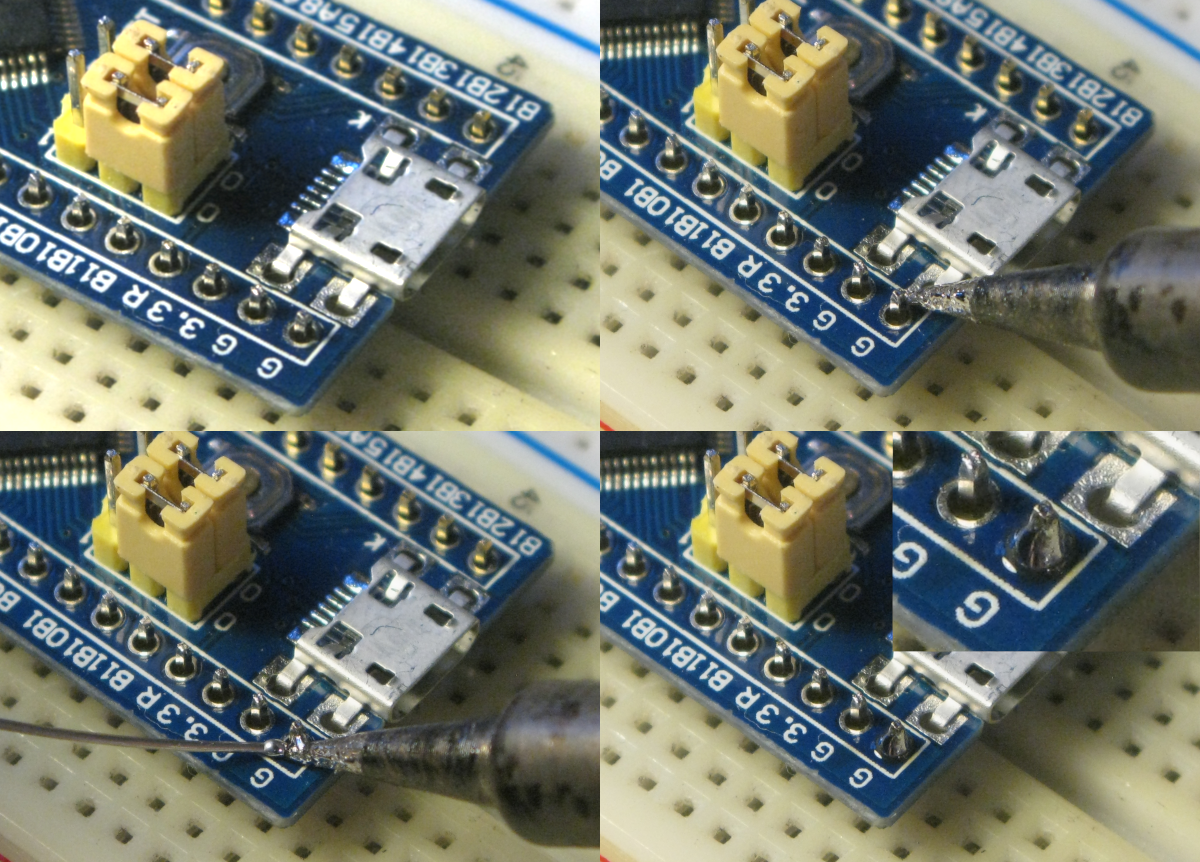
\includegraphics[width=0.99\textwidth,clip=true]{warsztat_elektroniczny/lutowanie}}\\
  \small
  \textbf{Lutowanie pinu mikrokontrolera.} Listwy kołkowe zostały umieszczone w płytce stykowej, aby je umiejscowić. \textit{Zaczynając od lewego górnego zdjęcia,
    zgodnie z ruchem wskazówek zegara:} Umiejscowienie pinu. Ogrzanie pinu i pola lutowniczego na płytce mikrokontrolera.
  Dotknięcie spoiwem (cyną).
  Gotowy lut (oraz jego przybliżenie).
\end{center}\end{Ramka}\end{figure}

Jeżeli Twój mikrokontroler nie ma przylutowanych pinów, musisz przylutować je sam/sama. Przymierz i odetnij
obcążkami dwa odcinki listwy kołkowej pasujące do otworów na brzegach płytki mikrokontrolera. Włóż piny do otworków
na płytce. Następnie odwiń lub wyciągnij odcinek cyny ze szpulki. Włącz lutownicę i odłóż ją na stojak. Jeżeli twoja lutownica
ma ustawianie temperatury, ustaw ją na około 250-300 st. C. Daj jej około minuty na osiągnięcie temperatury. Pamiętaj, że grot
lutownicy jest bardzo gorący. Lutownicę należy trzymać tylko i wyłącznie za rękojeść.
\\

Aby zalutować pin w otworze, najpierw dotknij grotem lutownicy
miejsca, które będziesz lutować (pola lutowniczego) oraz pinu. Trzeba ogrzać oba elementy przed ich połączeniem. Po około sekundzie, dotknij pinu końcówką odcinka cyny.
\\

Postaraj się, aby listwy kołkowe były prostopadle do płytki. Jeżeli masz odcinek damskiej listwy, możesz za jego pomocą
umiejscowić piny, które lutujesz. Możesz też użyć do tego płytki stykowej. Lutowanie zacznij od czterech pinów na rogach płytki.
\\

Kształt gotowego lutu powinien być stożkowaty. Jeżeli jest obły, oznacza to zbyt dużą ilość użytej cyny. Kuliste luty prawdopodobnie nie związały pinu z płytką (pole lutownicze nie było dobrze ogrzane). Jeśli lut nie jest błyszczący, oznacza to, że niepoprawnie związał (tzw. \textit{zimny lut}). W takim wypadku spróbuj dodać
topnika (np. kalafonii).\\

Umiejętne lutowanie wymaga trochę praktyki, ale nie jest skomplikowane. Pamiętaj, aby lutować w dobrze wentylowanym
pomieszczeniu. Po zakończeniu umyj ręce.

../stm32/01-przygotowanie.tex
\input{booklets-sections/warsztat/50-płytka_stykowa.tex}
\input{booklets-sections/warsztat/60-układy_scalone.tex}

\section{Wykład wideo}
\input{booklets-sections/warsztat/wykład-video.tex}

\copyrightFooter{
	© Matematyka dla Ciekawych Świata, 2020-2021.\\
	© Robert Ryszard Paciorek <rrp@opcode.eu.org>, 2020-2021.\\
	© Krzysztof Lasocki <krz.lasocki@gmail.com>, 2020-2021.\\
	Kopiowanie, modyfikowanie i redystrybucja dozwolone pod warunkiem zachowania informacji o autorach.
}

\end{document}
